\documentclass[1p]{elsarticle_modified}
%\bibliographystyle{elsarticle-num}

%\usepackage[colorlinks]{hyperref}
%\usepackage{abbrmath_seonhwa} %\Abb, \Ascr, \Acal ,\Abf, \Afrak
\usepackage{amsfonts}
\usepackage{amssymb}
\usepackage{amsmath}
\usepackage{amsthm}
\usepackage{scalefnt}
\usepackage{amsbsy}
\usepackage{kotex}
\usepackage{caption}
\usepackage{subfig}
\usepackage{color}
\usepackage{graphicx}
\usepackage{xcolor} %% white, black, red, green, blue, cyan, magenta, yellow
\usepackage{float}
\usepackage{setspace}
\usepackage{hyperref}

\usepackage{tikz}
\usetikzlibrary{arrows}

\usepackage{multirow}
\usepackage{array} % fixed length table
\usepackage{hhline}

%%%%%%%%%%%%%%%%%%%%%
\makeatletter
\renewcommand*\env@matrix[1][\arraystretch]{%
	\edef\arraystretch{#1}%
	\hskip -\arraycolsep
	\let\@ifnextchar\new@ifnextchar
	\array{*\c@MaxMatrixCols c}}
\makeatother %https://tex.stackexchange.com/questions/14071/how-can-i-increase-the-line-spacing-in-a-matrix
%%%%%%%%%%%%%%%

\usepackage[normalem]{ulem}

\newcommand{\msout}[1]{\ifmmode\text{\sout{\ensuremath{#1}}}\else\sout{#1}\fi}
%SOURCE: \msout is \stkout macro in https://tex.stackexchange.com/questions/20609/strikeout-in-math-mode

\newcommand{\cancel}[1]{
	\ifmmode
	{\color{red}\msout{#1}}
	\else
	{\color{red}\sout{#1}}
	\fi
}

\newcommand{\add}[1]{
	{\color{blue}\uwave{#1}}
}

\newcommand{\replace}[2]{
	\ifmmode
	{\color{red}\msout{#1}}{\color{blue}\uwave{#2}}
	\else
	{\color{red}\sout{#1}}{\color{blue}\uwave{#2}}
	\fi
}

\newcommand{\Sol}{\mathcal{S}} %segment
\newcommand{\D}{D} %diagram
\newcommand{\A}{\mathcal{A}} %arc


%%%%%%%%%%%%%%%%%%%%%%%%%%%%%5 test

\def\sl{\operatorname{\textup{SL}}(2,\Cbb)}
\def\psl{\operatorname{\textup{PSL}}(2,\Cbb)}
\def\quan{\mkern 1mu \triangleright \mkern 1mu}

\theoremstyle{definition}
\newtheorem{thm}{Theorem}[section]
\newtheorem{prop}[thm]{Proposition}
\newtheorem{lem}[thm]{Lemma}
\newtheorem{ques}[thm]{Question}
\newtheorem{cor}[thm]{Corollary}
\newtheorem{defn}[thm]{Definition}
\newtheorem{exam}[thm]{Example}
\newtheorem{rmk}[thm]{Remark}
\newtheorem{alg}[thm]{Algorithm}

\newcommand{\I}{\sqrt{-1}}
\begin{document}

%\begin{frontmatter}
%
%\title{Boundary parabolic representations of knots up to 8 crossings}
%
%%% Group authors per affiliation:
%\author{Yunhi Cho} 
%\address{Department of Mathematics, University of Seoul, Seoul, Korea}
%\ead{yhcho@uos.ac.kr}
%
%
%\author{Seonhwa Kim} %\fnref{s_kim}}
%\address{Center for Geometry and Physics, Institute for Basic Science, Pohang, 37673, Korea}
%\ead{ryeona17@ibs.re.kr}
%
%\author{Hyuk Kim}
%\address{Department of Mathematical Sciences, Seoul National University, Seoul 08826, Korea}
%\ead{hyukkim@snu.ac.kr}
%
%\author{Seokbeom Yoon}
%\address{Department of Mathematical Sciences, Seoul National University, Seoul, 08826,  Korea}
%\ead{sbyoon15@snu.ac.kr}
%
%\begin{abstract}
%We find all boundary parabolic representation of knots up to 8 crossings.
%
%\end{abstract}
%\begin{keyword}
%    \MSC[2010] 57M25 
%\end{keyword}
%
%\end{frontmatter}

%\linenumbers
%\tableofcontents
%
\newcommand\colored[1]{\textcolor{white}{\rule[-0.35ex]{0.8em}{1.4ex}}\kern-0.8em\color{red} #1}%
%\newcommand\colored[1]{\textcolor{white}{ #1}\kern-2.17ex	\textcolor{white}{ #1}\kern-1.81ex	\textcolor{white}{ #1}\kern-2.15ex\color{red}#1	}

{\Large $\underline{12n_{0705}~(K12n_{0705})}$}

\setlength{\tabcolsep}{10pt}
\renewcommand{\arraystretch}{1.6}
\vspace{1cm}\begin{tabular}{m{100pt}>{\centering\arraybackslash}m{274pt}}
\multirow{5}{120pt}{
	\centering
	\includegraphics[width=112pt]{../../../GIT/diagram.site/Diagrams/png/2794_12n_0705.png}\\
\ \ \ A knot diagram\footnotemark}&
\allowdisplaybreaks
\textbf{Linearized knot diagam} \\
\cline{2-2}
 &
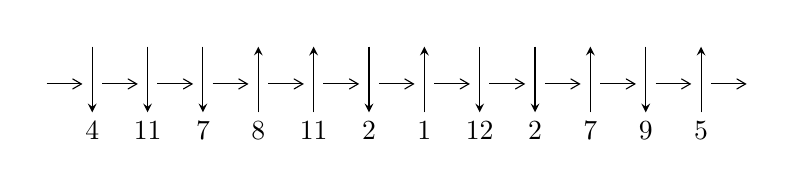
\begin{tikzpicture}[x=20pt, y=17pt]
	% nodes
	\node (C0) at (0, 0) {};
	\node (C1) at (1, 0) {};
	\node (C1U) at (1, +1) {};
	\node (C1D) at (1, -1) {4};

	\node (C2) at (2, 0) {};
	\node (C2U) at (2, +1) {};
	\node (C2D) at (2, -1) {11};

	\node (C3) at (3, 0) {};
	\node (C3U) at (3, +1) {};
	\node (C3D) at (3, -1) {7};

	\node (C4) at (4, 0) {};
	\node (C4U) at (4, +1) {};
	\node (C4D) at (4, -1) {8};

	\node (C5) at (5, 0) {};
	\node (C5U) at (5, +1) {};
	\node (C5D) at (5, -1) {11};

	\node (C6) at (6, 0) {};
	\node (C6U) at (6, +1) {};
	\node (C6D) at (6, -1) {2};

	\node (C7) at (7, 0) {};
	\node (C7U) at (7, +1) {};
	\node (C7D) at (7, -1) {1};

	\node (C8) at (8, 0) {};
	\node (C8U) at (8, +1) {};
	\node (C8D) at (8, -1) {12};

	\node (C9) at (9, 0) {};
	\node (C9U) at (9, +1) {};
	\node (C9D) at (9, -1) {2};

	\node (C10) at (10, 0) {};
	\node (C10U) at (10, +1) {};
	\node (C10D) at (10, -1) {7};

	\node (C11) at (11, 0) {};
	\node (C11U) at (11, +1) {};
	\node (C11D) at (11, -1) {9};

	\node (C12) at (12, 0) {};
	\node (C12U) at (12, +1) {};
	\node (C12D) at (12, -1) {5};
	\node (C13) at (13, 0) {};

	% arrows
	\draw[->,>={angle 60}]
	(C0) edge (C1) (C1) edge (C2) (C2) edge (C3) (C3) edge (C4) (C4) edge (C5) (C5) edge (C6) (C6) edge (C7) (C7) edge (C8) (C8) edge (C9) (C9) edge (C10) (C10) edge (C11) (C11) edge (C12) (C12) edge (C13) ;	\draw[->,>=stealth]
	(C1U) edge (C1D) (C2U) edge (C2D) (C3U) edge (C3D) (C4D) edge (C4U) (C5D) edge (C5U) (C6U) edge (C6D) (C7D) edge (C7U) (C8U) edge (C8D) (C9U) edge (C9D) (C10D) edge (C10U) (C11U) edge (C11D) (C12D) edge (C12U) ;
	\end{tikzpicture} \\
\hhline{~~} \\& 
\textbf{Solving Sequence} \\ \cline{2-2} 
 &
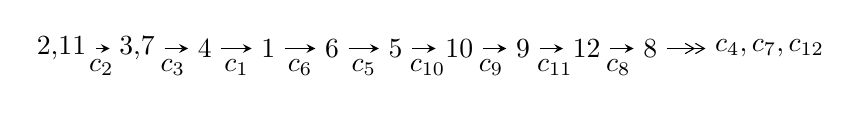
\begin{tikzpicture}[x=23pt, y=7pt]
	% node
	\node (A0) at (-1/8, 0) {2,11};
	\node (A1) at (17/16, 0) {3,7};
	\node (A2) at (17/8, 0) {4};
	\node (A3) at (25/8, 0) {1};
	\node (A4) at (33/8, 0) {6};
	\node (A5) at (41/8, 0) {5};
	\node (A6) at (49/8, 0) {10};
	\node (A7) at (57/8, 0) {9};
	\node (A8) at (65/8, 0) {12};
	\node (A9) at (73/8, 0) {8};
	\node (C1) at (1/2, -1) {$c_{2}$};
	\node (C2) at (13/8, -1) {$c_{3}$};
	\node (C3) at (21/8, -1) {$c_{1}$};
	\node (C4) at (29/8, -1) {$c_{6}$};
	\node (C5) at (37/8, -1) {$c_{5}$};
	\node (C6) at (45/8, -1) {$c_{10}$};
	\node (C7) at (53/8, -1) {$c_{9}$};
	\node (C8) at (61/8, -1) {$c_{11}$};
	\node (C9) at (69/8, -1) {$c_{8}$};
	\node (A10) at (11, 0) {$c_{4},c_{7},c_{12}$};

	% edge
	\draw[->,>=stealth]	
	(A0) edge (A1) (A1) edge (A2) (A2) edge (A3) (A3) edge (A4) (A4) edge (A5) (A5) edge (A6) (A6) edge (A7) (A7) edge (A8) (A8) edge (A9) ;
	\draw[->>,>={angle 60}]	
	(A9) edge (A10);
\end{tikzpicture} \\ 

\end{tabular} \\

\footnotetext{
The image of knot diagram is generated by the software ``\textbf{Draw programme}" developed by Andrew Bartholomew(\url{http://www.layer8.co.uk/maths/draw/index.htm\#Running-draw}), where we modified some parts for our purpose(\url{https://github.com/CATsTAILs/LinksPainter}).
}\phantom \\ \newline 
\centering \textbf{Ideals for irreducible components\footnotemark of $X_{\text{par}}$} 
 
\begin{align*}
I^u_{1}&=\langle 
2.19181\times10^{382} u^{75}+6.42258\times10^{381} u^{74}+\cdots+4.60404\times10^{387} b+1.33471\times10^{388},\\
\phantom{I^u_{1}}&\phantom{= \langle  }-2.21394\times10^{388} u^{75}+1.64912\times10^{388} u^{74}+\cdots+7.19321\times10^{392} a-4.98498\times10^{393},\\
\phantom{I^u_{1}}&\phantom{= \langle  }u^{76}- u^{75}+\cdots-23760 u+74007\rangle \\
I^u_{2}&=\langle 
-149224377175319 u^{21}+98709240274610 u^{20}+\cdots+96703178408689 b-82488765402898,\\
\phantom{I^u_{2}}&\phantom{= \langle  }360716486705467 u^{21}-113938156490740 u^{20}+\cdots+96703178408689 a+729010725759272,\\
\phantom{I^u_{2}}&\phantom{= \langle  }u^{22}+6 u^{20}+\cdots+3 u+1\rangle \\
\\
\end{align*}
\raggedright * 2 irreducible components of $\dim_{\mathbb{C}}=0$, with total 98 representations.\\
\footnotetext{All coefficients of polynomials are rational numbers. But the coefficients are sometimes approximated in decimal forms when there is not enough margin.}
\newpage
\renewcommand{\arraystretch}{1}
\centering \section*{I. $I^u_{1}= \langle 2.19\times10^{382} u^{75}+6.42\times10^{381} u^{74}+\cdots+4.60\times10^{387} b+1.33\times10^{388},\;-2.21\times10^{388} u^{75}+1.65\times10^{388} u^{74}+\cdots+7.19\times10^{392} a-4.98\times10^{393},\;u^{76}- u^{75}+\cdots-23760 u+74007 \rangle$}
\flushleft \textbf{(i) Arc colorings}\\
\begin{tabular}{m{7pt} m{180pt} m{7pt} m{180pt} }
\flushright $a_{2}=$&$\begin{pmatrix}1\\0\end{pmatrix}$ \\
\flushright $a_{11}=$&$\begin{pmatrix}0\\u\end{pmatrix}$ \\
\flushright $a_{3}=$&$\begin{pmatrix}1\\u^2\end{pmatrix}$ \\
\flushright $a_{7}=$&$\begin{pmatrix}0.0000307782 u^{75}-0.0000229260 u^{74}+\cdots+20.3789 u+6.93012\\-4.76062\times10^{-6} u^{75}-1.39499\times10^{-6} u^{74}+\cdots-0.757161 u-2.89899\end{pmatrix}$ \\
\flushright $a_{4}=$&$\begin{pmatrix}-7.78630\times10^{-6} u^{75}-1.40375\times10^{-6} u^{74}+\cdots+0.0566661 u-7.56840\\-9.12142\times10^{-6} u^{75}+8.62552\times10^{-6} u^{74}+\cdots-5.37177 u+1.51302\end{pmatrix}$ \\
\flushright $a_{1}=$&$\begin{pmatrix}-0.0000221139 u^{75}+0.0000317720 u^{74}+\cdots-22.3602 u+6.91672\\6.38702\times10^{-6} u^{75}-3.29061\times10^{-6} u^{74}+\cdots+6.79986 u+0.825307\end{pmatrix}$ \\
\flushright $a_{6}=$&$\begin{pmatrix}0.0000260176 u^{75}-0.0000243210 u^{74}+\cdots+19.6217 u+4.03113\\-4.76062\times10^{-6} u^{75}-1.39499\times10^{-6} u^{74}+\cdots-0.757161 u-2.89899\end{pmatrix}$ \\
\flushright $a_{5}=$&$\begin{pmatrix}0.0000260176 u^{75}-0.0000243210 u^{74}+\cdots+19.6217 u+4.03113\\-6.93011\times10^{-6} u^{75}+1.21906\times10^{-6} u^{74}+\cdots-2.64233 u-3.02455\end{pmatrix}$ \\
\flushright $a_{10}=$&$\begin{pmatrix}-6.72650\times10^{-6} u^{75}+0.0000218094 u^{74}+\cdots-13.5272 u+11.5689\\8.76516\times10^{-6} u^{75}-0.0000117617 u^{74}+\cdots+10.6096 u-1.69248\end{pmatrix}$ \\
\flushright $a_{9}=$&$\begin{pmatrix}2.03866\times10^{-6} u^{75}+0.0000100477 u^{74}+\cdots-2.91766 u+9.87645\\8.76516\times10^{-6} u^{75}-0.0000117617 u^{74}+\cdots+10.6096 u-1.69248\end{pmatrix}$ \\
\flushright $a_{12}=$&$\begin{pmatrix}-0.0000523639 u^{75}+0.0000528643 u^{74}+\cdots-39.9625 u-1.49577\\8.63617\times10^{-6} u^{75}-3.40978\times10^{-6} u^{74}+\cdots+3.57479 u+4.99056\end{pmatrix}$ \\
\flushright $a_{8}=$&$\begin{pmatrix}0.0000265357 u^{75}-0.0000320384 u^{74}+\cdots+27.2940 u-5.37665\\-0.0000162618 u^{75}+0.0000181990 u^{74}+\cdots-12.7453 u+0.0118103\end{pmatrix}$\\&\end{tabular}
\flushleft \textbf{(ii) Obstruction class $= -1$}\\~\\
\flushleft \textbf{(iii) Cusp Shapes $= 0.0000191588 u^{75}-0.0000387698 u^{74}+\cdots-0.636809 u-2.73074$}\\~\\
\newpage\renewcommand{\arraystretch}{1}
\flushleft \textbf{(iv) u-Polynomials at the component}\newline \\
\begin{tabular}{m{50pt}|m{274pt}}
Crossings & \hspace{64pt}u-Polynomials at each crossing \\
\hline $$\begin{aligned}c_{1}\end{aligned}$$&$\begin{aligned}
&u^{76}-10 u^{75}+\cdots-221 u+17
\end{aligned}$\\
\hline $$\begin{aligned}c_{2}\end{aligned}$$&$\begin{aligned}
&u^{76}- u^{75}+\cdots-23760 u+74007
\end{aligned}$\\
\hline $$\begin{aligned}c_{3}\end{aligned}$$&$\begin{aligned}
&u^{76}+2 u^{75}+\cdots-19464 u+3677
\end{aligned}$\\
\hline $$\begin{aligned}c_{4}\end{aligned}$$&$\begin{aligned}
&u^{76}-2 u^{75}+\cdots+549 u+207
\end{aligned}$\\
\hline $$\begin{aligned}c_{5}\end{aligned}$$&$\begin{aligned}
&u^{76}- u^{75}+\cdots+34842166 u+3425393
\end{aligned}$\\
\hline $$\begin{aligned}c_{6}\end{aligned}$$&$\begin{aligned}
&u^{76}+53 u^{74}+\cdots+7437 u+763
\end{aligned}$\\
\hline $$\begin{aligned}c_{7}\end{aligned}$$&$\begin{aligned}
&u^{76}-7 u^{75}+\cdots+27 u+1
\end{aligned}$\\
\hline $$\begin{aligned}c_{8},c_{11}\end{aligned}$$&$\begin{aligned}
&u^{76}-9 u^{75}+\cdots-362 u+19
\end{aligned}$\\
\hline $$\begin{aligned}c_{9}\end{aligned}$$&$\begin{aligned}
&u^{76}-8 u^{75}+\cdots+57253563 u+3204791
\end{aligned}$\\
\hline $$\begin{aligned}c_{10}\end{aligned}$$&$\begin{aligned}
&u^{76}-9 u^{75}+\cdots-530 u+1279
\end{aligned}$\\
\hline $$\begin{aligned}c_{12}\end{aligned}$$&$\begin{aligned}
&u^{76}-6 u^{75}+\cdots+78 u+35
\end{aligned}$\\
\hline
\end{tabular}\\~\\
\newpage\renewcommand{\arraystretch}{1}
\flushleft \textbf{(v) Riley Polynomials at the component}\newline \\
\begin{tabular}{m{50pt}|m{274pt}}
Crossings & \hspace{64pt}Riley Polynomials at each crossing \\
\hline $$\begin{aligned}c_{1}\end{aligned}$$&$\begin{aligned}
&y^{76}+18 y^{75}+\cdots-2227 y+289
\end{aligned}$\\
\hline $$\begin{aligned}c_{2}\end{aligned}$$&$\begin{aligned}
&y^{76}+93 y^{75}+\cdots+236846070036 y+5477036049
\end{aligned}$\\
\hline $$\begin{aligned}c_{3}\end{aligned}$$&$\begin{aligned}
&y^{76}+20 y^{75}+\cdots+475032998 y+13520329
\end{aligned}$\\
\hline $$\begin{aligned}c_{4}\end{aligned}$$&$\begin{aligned}
&y^{76}-14 y^{75}+\cdots-1120293 y+42849
\end{aligned}$\\
\hline $$\begin{aligned}c_{5}\end{aligned}$$&$\begin{aligned}
&y^{76}-57 y^{75}+\cdots-439239317966814 y+11733317204449
\end{aligned}$\\
\hline $$\begin{aligned}c_{6}\end{aligned}$$&$\begin{aligned}
&y^{76}+106 y^{75}+\cdots+5285439 y+582169
\end{aligned}$\\
\hline $$\begin{aligned}c_{7}\end{aligned}$$&$\begin{aligned}
&y^{76}+15 y^{75}+\cdots-7 y+1
\end{aligned}$\\
\hline $$\begin{aligned}c_{8},c_{11}\end{aligned}$$&$\begin{aligned}
&y^{76}+63 y^{75}+\cdots+208 y+361
\end{aligned}$\\
\hline $$\begin{aligned}c_{9}\end{aligned}$$&$\begin{aligned}
&y^{76}+128 y^{75}+\cdots+7840289593898607 y+10270685353681
\end{aligned}$\\
\hline $$\begin{aligned}c_{10}\end{aligned}$$&$\begin{aligned}
&y^{76}-105 y^{75}+\cdots-4524622 y+1635841
\end{aligned}$\\
\hline $$\begin{aligned}c_{12}\end{aligned}$$&$\begin{aligned}
&y^{76}-8 y^{75}+\cdots-58374 y+1225
\end{aligned}$\\
\hline
\end{tabular}\\~\\
\newpage\flushleft \textbf{(vi) Complex Volumes and Cusp Shapes}
$$\begin{array}{c|c|c}  
\text{Solutions to }I^u_{1}& \I (\text{vol} + \sqrt{-1}CS) & \text{Cusp shape}\\
 \hline 
\begin{aligned}
u &= \phantom{-}1.009200 + 0.019949 I \\
a &= -0.755402 + 0.769566 I \\
b &= -0.141359 - 0.446045 I\end{aligned}
 & \phantom{-}0.24108 - 3.09498 I & -7.87234 + 7.34515 I \\ \hline\begin{aligned}
u &= \phantom{-}1.009200 - 0.019949 I \\
a &= -0.755402 - 0.769566 I \\
b &= -0.141359 + 0.446045 I\end{aligned}
 & \phantom{-}0.24108 + 3.09498 I & -7.87234 - 7.34515 I \\ \hline\begin{aligned}
u &= -0.165558 + 0.962769 I \\
a &= -0.682721 + 0.385052 I \\
b &= -0.846371 - 0.090077 I\end{aligned}
 & -1.18877 + 0.93128 I & -6.34635 - 7.99915 I \\ \hline\begin{aligned}
u &= -0.165558 - 0.962769 I \\
a &= -0.682721 - 0.385052 I \\
b &= -0.846371 + 0.090077 I\end{aligned}
 & -1.18877 - 0.93128 I & -6.34635 + 7.99915 I \\ \hline\begin{aligned}
u &= -0.895115 + 0.388201 I \\
a &= -0.560008 + 0.114830 I \\
b &= -0.259160 + 0.201495 I\end{aligned}
 & -1.46389 + 0.73897 I & -3.77155 + 0. I\phantom{ +0.000000I} \\ \hline\begin{aligned}
u &= -0.895115 - 0.388201 I \\
a &= -0.560008 - 0.114830 I \\
b &= -0.259160 - 0.201495 I\end{aligned}
 & -1.46389 - 0.73897 I & -3.77155 + 0. I\phantom{ +0.000000I} \\ \hline\begin{aligned}
u &= \phantom{-}0.810100 + 0.696527 I \\
a &= -0.338242 + 0.436580 I \\
b &= \phantom{-}0.218121 + 0.101852 I\end{aligned}
 & \phantom{-}4.06725 - 2.79115 I & \phantom{-0.000000 } 0 \\ \hline\begin{aligned}
u &= \phantom{-}0.810100 - 0.696527 I \\
a &= -0.338242 - 0.436580 I \\
b &= \phantom{-}0.218121 - 0.101852 I\end{aligned}
 & \phantom{-}4.06725 + 2.79115 I & \phantom{-0.000000 } 0 \\ \hline\begin{aligned}
u &= \phantom{-}0.564725 + 0.948830 I \\
a &= -0.645295 - 0.262477 I \\
b &= \phantom{-}0.150567 - 0.619486 I\end{aligned}
 & \phantom{-}3.85710 - 3.89576 I & \phantom{-0.000000 } 0 \\ \hline\begin{aligned}
u &= \phantom{-}0.564725 - 0.948830 I \\
a &= -0.645295 + 0.262477 I \\
b &= \phantom{-}0.150567 + 0.619486 I\end{aligned}
 & \phantom{-}3.85710 + 3.89576 I & \phantom{-0.000000 } 0\\
 \hline 
 \end{array}$$\newpage$$\begin{array}{c|c|c}  
\text{Solutions to }I^u_{1}& \I (\text{vol} + \sqrt{-1}CS) & \text{Cusp shape}\\
 \hline 
\begin{aligned}
u &= \phantom{-}0.046617 + 1.142370 I \\
a &= -0.63482 + 2.26238 I \\
b &= \phantom{-}0.79960 - 2.66733 I\end{aligned}
 & \phantom{-}4.62267 + 0.14372 I & \phantom{-0.000000 } 0 \\ \hline\begin{aligned}
u &= \phantom{-}0.046617 - 1.142370 I \\
a &= -0.63482 - 2.26238 I \\
b &= \phantom{-}0.79960 + 2.66733 I\end{aligned}
 & \phantom{-}4.62267 - 0.14372 I & \phantom{-0.000000 } 0 \\ \hline\begin{aligned}
u &= \phantom{-}1.150780 + 0.219130 I \\
a &= \phantom{-}0.522685 + 0.399011 I \\
b &= -0.094055 - 0.540195 I\end{aligned}
 & -0.65964 - 4.41450 I & \phantom{-0.000000 } 0 \\ \hline\begin{aligned}
u &= \phantom{-}1.150780 - 0.219130 I \\
a &= \phantom{-}0.522685 - 0.399011 I \\
b &= -0.094055 + 0.540195 I\end{aligned}
 & -0.65964 + 4.41450 I & \phantom{-0.000000 } 0 \\ \hline\begin{aligned}
u &= -0.592031 + 0.568502 I \\
a &= \phantom{-}1.33340 - 0.84287 I \\
b &= -0.193442 + 0.277813 I\end{aligned}
 & -1.42596 - 3.59118 I & -1.75527 + 3.21770 I \\ \hline\begin{aligned}
u &= -0.592031 - 0.568502 I \\
a &= \phantom{-}1.33340 + 0.84287 I \\
b &= -0.193442 - 0.277813 I\end{aligned}
 & -1.42596 + 3.59118 I & -1.75527 - 3.21770 I \\ \hline\begin{aligned}
u &= \phantom{-}1.164960 + 0.183393 I \\
a &= -0.472076 + 0.327161 I \\
b &= -1.356770 + 0.193388 I\end{aligned}
 & \phantom{-}0.967603 - 0.985142 I & \phantom{-0.000000 } 0 \\ \hline\begin{aligned}
u &= \phantom{-}1.164960 - 0.183393 I \\
a &= -0.472076 - 0.327161 I \\
b &= -1.356770 - 0.193388 I\end{aligned}
 & \phantom{-}0.967603 + 0.985142 I & \phantom{-0.000000 } 0 \\ \hline\begin{aligned}
u &= -0.520526 + 0.633146 I \\
a &= -0.375631 + 0.423504 I \\
b &= \phantom{-}1.47986 + 0.80086 I\end{aligned}
 & \phantom{-}2.52872 - 8.60121 I & \phantom{-}1.83866 + 3.84455 I \\ \hline\begin{aligned}
u &= -0.520526 - 0.633146 I \\
a &= -0.375631 - 0.423504 I \\
b &= \phantom{-}1.47986 - 0.80086 I\end{aligned}
 & \phantom{-}2.52872 + 8.60121 I & \phantom{-}1.83866 - 3.84455 I\\
 \hline 
 \end{array}$$\newpage$$\begin{array}{c|c|c}  
\text{Solutions to }I^u_{1}& \I (\text{vol} + \sqrt{-1}CS) & \text{Cusp shape}\\
 \hline 
\begin{aligned}
u &= \phantom{-}0.294916 + 0.746389 I \\
a &= \phantom{-}1.98912 - 0.26808 I \\
b &= -0.433848 - 0.020928 I\end{aligned}
 & \phantom{-}3.01635 + 9.32304 I & \phantom{-}3.19894 - 5.62741 I \\ \hline\begin{aligned}
u &= \phantom{-}0.294916 - 0.746389 I \\
a &= \phantom{-}1.98912 + 0.26808 I \\
b &= -0.433848 + 0.020928 I\end{aligned}
 & \phantom{-}3.01635 - 9.32304 I & \phantom{-}3.19894 + 5.62741 I \\ \hline\begin{aligned}
u &= -0.771153 + 0.130660 I \\
a &= -1.040020 - 0.437054 I \\
b &= -0.083499 - 0.951857 I\end{aligned}
 & \phantom{-}4.69688 - 2.57649 I & \phantom{-}1.57467 + 2.30402 I \\ \hline\begin{aligned}
u &= -0.771153 - 0.130660 I \\
a &= -1.040020 + 0.437054 I \\
b &= -0.083499 + 0.951857 I\end{aligned}
 & \phantom{-}4.69688 + 2.57649 I & \phantom{-}1.57467 - 2.30402 I \\ \hline\begin{aligned}
u &= \phantom{-}0.131578 + 0.739838 I \\
a &= -1.68627 - 0.52919 I \\
b &= \phantom{-}1.321970 - 0.419785 I\end{aligned}
 & \phantom{-}4.44676 + 0.47633 I & \phantom{-}7.82049 - 1.23300 I \\ \hline\begin{aligned}
u &= \phantom{-}0.131578 - 0.739838 I \\
a &= -1.68627 + 0.52919 I \\
b &= \phantom{-}1.321970 + 0.419785 I\end{aligned}
 & \phantom{-}4.44676 - 0.47633 I & \phantom{-}7.82049 + 1.23300 I \\ \hline\begin{aligned}
u &= -0.365970 + 0.650492 I \\
a &= -0.923300 + 0.352826 I \\
b &= -0.405458 + 0.239034 I\end{aligned}
 & -1.30459 + 1.15321 I & -3.91266 - 5.89962 I \\ \hline\begin{aligned}
u &= -0.365970 - 0.650492 I \\
a &= -0.923300 - 0.352826 I \\
b &= -0.405458 - 0.239034 I\end{aligned}
 & -1.30459 - 1.15321 I & -3.91266 + 5.89962 I \\ \hline\begin{aligned}
u &= \phantom{-}0.027626 + 1.265550 I \\
a &= -0.18747 + 1.64404 I \\
b &= \phantom{-}0.41367 - 2.13372 I\end{aligned}
 & \phantom{-}4.64117 + 0.14396 I & \phantom{-0.000000 } 0 \\ \hline\begin{aligned}
u &= \phantom{-}0.027626 - 1.265550 I \\
a &= -0.18747 - 1.64404 I \\
b &= \phantom{-}0.41367 + 2.13372 I\end{aligned}
 & \phantom{-}4.64117 - 0.14396 I & \phantom{-0.000000 } 0\\
 \hline 
 \end{array}$$\newpage$$\begin{array}{c|c|c}  
\text{Solutions to }I^u_{1}& \I (\text{vol} + \sqrt{-1}CS) & \text{Cusp shape}\\
 \hline 
\begin{aligned}
u &= -1.050630 + 0.743716 I \\
a &= -0.260234 - 0.008456 I \\
b &= -1.151120 - 0.614051 I\end{aligned}
 & -0.025364 - 0.694709 I & \phantom{-0.000000 } 0 \\ \hline\begin{aligned}
u &= -1.050630 - 0.743716 I \\
a &= -0.260234 + 0.008456 I \\
b &= -1.151120 + 0.614051 I\end{aligned}
 & -0.025364 + 0.694709 I & \phantom{-0.000000 } 0 \\ \hline\begin{aligned}
u &= \phantom{-}0.966250 + 0.854364 I \\
a &= \phantom{-}0.030557 + 0.171811 I \\
b &= \phantom{-}0.284472 - 0.438444 I\end{aligned}
 & \phantom{-}4.18587 - 3.26120 I & \phantom{-0.000000 } 0 \\ \hline\begin{aligned}
u &= \phantom{-}0.966250 - 0.854364 I \\
a &= \phantom{-}0.030557 - 0.171811 I \\
b &= \phantom{-}0.284472 + 0.438444 I\end{aligned}
 & \phantom{-}4.18587 + 3.26120 I & \phantom{-0.000000 } 0 \\ \hline\begin{aligned}
u &= -0.030321 + 0.608824 I \\
a &= -0.377141 - 0.458763 I \\
b &= \phantom{-}1.236080 - 0.334684 I\end{aligned}
 & -1.19917 + 5.41165 I & \phantom{-}1.34156 - 7.26392 I \\ \hline\begin{aligned}
u &= -0.030321 - 0.608824 I \\
a &= -0.377141 + 0.458763 I \\
b &= \phantom{-}1.236080 + 0.334684 I\end{aligned}
 & -1.19917 - 5.41165 I & \phantom{-}1.34156 + 7.26392 I \\ \hline\begin{aligned}
u &= \phantom{-}0.356043 + 0.423213 I \\
a &= -2.08467 - 0.32556 I \\
b &= -0.069706 + 0.303853 I\end{aligned}
 & \phantom{-}0.24691 + 2.62762 I & \phantom{-}0.32414 - 5.86582 I \\ \hline\begin{aligned}
u &= \phantom{-}0.356043 - 0.423213 I \\
a &= -2.08467 + 0.32556 I \\
b &= -0.069706 - 0.303853 I\end{aligned}
 & \phantom{-}0.24691 - 2.62762 I & \phantom{-}0.32414 + 5.86582 I \\ \hline\begin{aligned}
u &= -0.24387 + 1.47515 I \\
a &= \phantom{-}0.017377 - 1.220120 I \\
b &= \phantom{-}0.44822 + 1.78089 I\end{aligned}
 & \phantom{-}11.22230 + 0.28649 I & \phantom{-0.000000 } 0 \\ \hline\begin{aligned}
u &= -0.24387 - 1.47515 I \\
a &= \phantom{-}0.017377 + 1.220120 I \\
b &= \phantom{-}0.44822 - 1.78089 I\end{aligned}
 & \phantom{-}11.22230 - 0.28649 I & \phantom{-0.000000 } 0\\
 \hline 
 \end{array}$$\newpage$$\begin{array}{c|c|c}  
\text{Solutions to }I^u_{1}& \I (\text{vol} + \sqrt{-1}CS) & \text{Cusp shape}\\
 \hline 
\begin{aligned}
u &= -0.327271 + 0.358349 I \\
a &= -0.886714 - 0.274566 I \\
b &= -1.045100 + 0.416367 I\end{aligned}
 & -1.90605 + 1.11051 I & \phantom{-}2.44459 + 0.53234 I \\ \hline\begin{aligned}
u &= -0.327271 - 0.358349 I \\
a &= -0.886714 + 0.274566 I \\
b &= -1.045100 - 0.416367 I\end{aligned}
 & -1.90605 - 1.11051 I & \phantom{-}2.44459 - 0.53234 I \\ \hline\begin{aligned}
u &= -1.42583 + 0.57546 I \\
a &= \phantom{-}0.498504 + 0.022033 I \\
b &= \phantom{-}0.479276 + 0.563280 I\end{aligned}
 & \phantom{-}4.46008 + 9.11025 I & \phantom{-0.000000 } 0 \\ \hline\begin{aligned}
u &= -1.42583 - 0.57546 I \\
a &= \phantom{-}0.498504 - 0.022033 I \\
b &= \phantom{-}0.479276 - 0.563280 I\end{aligned}
 & \phantom{-}4.46008 - 9.11025 I & \phantom{-0.000000 } 0 \\ \hline\begin{aligned}
u &= \phantom{-}0.250236 + 0.342228 I \\
a &= -1.226160 + 0.462405 I \\
b &= \phantom{-}0.309303 + 0.470318 I\end{aligned}
 & \phantom{-}1.39381 + 0.89309 I & \phantom{-}4.09738 - 0.87482 I \\ \hline\begin{aligned}
u &= \phantom{-}0.250236 - 0.342228 I \\
a &= -1.226160 - 0.462405 I \\
b &= \phantom{-}0.309303 - 0.470318 I\end{aligned}
 & \phantom{-}1.39381 - 0.89309 I & \phantom{-}4.09738 + 0.87482 I \\ \hline\begin{aligned}
u &= -0.30462 + 1.58289 I \\
a &= -0.159862 - 0.920028 I \\
b &= -0.20723 + 1.71520 I\end{aligned}
 & \phantom{-}3.23935 + 3.92724 I & \phantom{-0.000000 } 0 \\ \hline\begin{aligned}
u &= -0.30462 - 1.58289 I \\
a &= -0.159862 + 0.920028 I \\
b &= -0.20723 - 1.71520 I\end{aligned}
 & \phantom{-}3.23935 - 3.92724 I & \phantom{-0.000000 } 0 \\ \hline\begin{aligned}
u &= \phantom{-}0.44818 + 1.58154 I \\
a &= \phantom{-}0.414772 - 0.918491 I \\
b &= \phantom{-}0.52106 + 1.85961 I\end{aligned}
 & \phantom{-}11.27930 - 1.44429 I & \phantom{-0.000000 } 0 \\ \hline\begin{aligned}
u &= \phantom{-}0.44818 - 1.58154 I \\
a &= \phantom{-}0.414772 + 0.918491 I \\
b &= \phantom{-}0.52106 - 1.85961 I\end{aligned}
 & \phantom{-}11.27930 + 1.44429 I & \phantom{-0.000000 } 0\\
 \hline 
 \end{array}$$\newpage$$\begin{array}{c|c|c}  
\text{Solutions to }I^u_{1}& \I (\text{vol} + \sqrt{-1}CS) & \text{Cusp shape}\\
 \hline 
\begin{aligned}
u &= -0.017872 + 0.303347 I \\
a &= \phantom{-}3.82605 + 1.87714 I \\
b &= -1.132580 + 0.363636 I\end{aligned}
 & \phantom{-}3.42718 - 1.06387 I & \phantom{-}2.11989 - 0.34485 I \\ \hline\begin{aligned}
u &= -0.017872 - 0.303347 I \\
a &= \phantom{-}3.82605 - 1.87714 I \\
b &= -1.132580 - 0.363636 I\end{aligned}
 & \phantom{-}3.42718 + 1.06387 I & \phantom{-}2.11989 + 0.34485 I \\ \hline\begin{aligned}
u &= \phantom{-}0.25994 + 1.72565 I \\
a &= \phantom{-}0.109906 + 1.123310 I \\
b &= -0.39160 - 2.11059 I\end{aligned}
 & \phantom{-}12.4056 - 6.9129 I & \phantom{-0.000000 } 0 \\ \hline\begin{aligned}
u &= \phantom{-}0.25994 - 1.72565 I \\
a &= \phantom{-}0.109906 - 1.123310 I \\
b &= -0.39160 + 2.11059 I\end{aligned}
 & \phantom{-}12.4056 + 6.9129 I & \phantom{-0.000000 } 0 \\ \hline\begin{aligned}
u &= \phantom{-}0.27832 + 1.76522 I \\
a &= \phantom{-}0.022137 - 1.136350 I \\
b &= \phantom{-}0.43502 + 1.99701 I\end{aligned}
 & \phantom{-}13.3454 - 7.9741 I & \phantom{-0.000000 } 0 \\ \hline\begin{aligned}
u &= \phantom{-}0.27832 - 1.76522 I \\
a &= \phantom{-}0.022137 + 1.136350 I \\
b &= \phantom{-}0.43502 - 1.99701 I\end{aligned}
 & \phantom{-}13.3454 + 7.9741 I & \phantom{-0.000000 } 0 \\ \hline\begin{aligned}
u &= \phantom{-}0.54424 + 1.73484 I \\
a &= -0.126901 + 1.035400 I \\
b &= -0.05331 - 1.76815 I\end{aligned}
 & \phantom{-}6.10244 - 3.92680 I & \phantom{-0.000000 } 0 \\ \hline\begin{aligned}
u &= \phantom{-}0.54424 - 1.73484 I \\
a &= -0.126901 - 1.035400 I \\
b &= -0.05331 + 1.76815 I\end{aligned}
 & \phantom{-}6.10244 + 3.92680 I & \phantom{-0.000000 } 0 \\ \hline\begin{aligned}
u &= -0.08745 + 1.81957 I \\
a &= \phantom{-}0.183051 - 0.960988 I \\
b &= -0.02671 + 1.86706 I\end{aligned}
 & \phantom{-}8.17378 + 5.03717 I & \phantom{-0.000000 } 0 \\ \hline\begin{aligned}
u &= -0.08745 - 1.81957 I \\
a &= \phantom{-}0.183051 + 0.960988 I \\
b &= -0.02671 - 1.86706 I\end{aligned}
 & \phantom{-}8.17378 - 5.03717 I & \phantom{-0.000000 } 0\\
 \hline 
 \end{array}$$\newpage$$\begin{array}{c|c|c}  
\text{Solutions to }I^u_{1}& \I (\text{vol} + \sqrt{-1}CS) & \text{Cusp shape}\\
 \hline 
\begin{aligned}
u &= \phantom{-}0.44832 + 1.79678 I \\
a &= \phantom{-}0.011918 - 1.072770 I \\
b &= \phantom{-}0.23871 + 1.75816 I\end{aligned}
 & \phantom{-}6.36319 - 10.94220 I & \phantom{-0.000000 } 0 \\ \hline\begin{aligned}
u &= \phantom{-}0.44832 - 1.79678 I \\
a &= \phantom{-}0.011918 + 1.072770 I \\
b &= \phantom{-}0.23871 - 1.75816 I\end{aligned}
 & \phantom{-}6.36319 + 10.94220 I & \phantom{-0.000000 } 0 \\ \hline\begin{aligned}
u &= \phantom{-}0.33240 + 1.86146 I \\
a &= -0.052763 + 0.804686 I \\
b &= -0.52702 - 2.08999 I\end{aligned}
 & \phantom{-}8.73089 - 7.50113 I & \phantom{-0.000000 } 0 \\ \hline\begin{aligned}
u &= \phantom{-}0.33240 - 1.86146 I \\
a &= -0.052763 - 0.804686 I \\
b &= -0.52702 + 2.08999 I\end{aligned}
 & \phantom{-}8.73089 + 7.50113 I & \phantom{-0.000000 } 0 \\ \hline\begin{aligned}
u &= -0.48571 + 1.83508 I \\
a &= -0.079389 + 1.054680 I \\
b &= -0.17441 - 1.45972 I\end{aligned}
 & \phantom{-}8.82884 + 2.54421 I & \phantom{-0.000000 } 0 \\ \hline\begin{aligned}
u &= -0.48571 - 1.83508 I \\
a &= -0.079389 - 1.054680 I \\
b &= -0.17441 + 1.45972 I\end{aligned}
 & \phantom{-}8.82884 - 2.54421 I & \phantom{-0.000000 } 0 \\ \hline\begin{aligned}
u &= -0.12198 + 1.91973 I \\
a &= -0.088250 + 1.035080 I \\
b &= \phantom{-}0.07581 - 1.61679 I\end{aligned}
 & \phantom{-}8.04212 + 1.07975 I & \phantom{-0.000000 } 0 \\ \hline\begin{aligned}
u &= -0.12198 - 1.91973 I \\
a &= -0.088250 - 1.035080 I \\
b &= \phantom{-}0.07581 + 1.61679 I\end{aligned}
 & \phantom{-}8.04212 - 1.07975 I & \phantom{-0.000000 } 0 \\ \hline\begin{aligned}
u &= -0.53576 + 1.86215 I \\
a &= \phantom{-}0.079592 + 1.028730 I \\
b &= \phantom{-}0.39767 - 2.06815 I\end{aligned}
 & \phantom{-}12.2627 + 16.8504 I & \phantom{-0.000000 } 0 \\ \hline\begin{aligned}
u &= -0.53576 - 1.86215 I \\
a &= \phantom{-}0.079592 - 1.028730 I \\
b &= \phantom{-}0.39767 + 2.06815 I\end{aligned}
 & \phantom{-}12.2627 - 16.8504 I & \phantom{-0.000000 } 0\\
 \hline 
 \end{array}$$\newpage$$\begin{array}{c|c|c}  
\text{Solutions to }I^u_{1}& \I (\text{vol} + \sqrt{-1}CS) & \text{Cusp shape}\\
 \hline 
\begin{aligned}
u &= \phantom{-}0.12813 + 2.03521 I \\
a &= -0.082429 - 0.921487 I \\
b &= -0.36312 + 1.77545 I\end{aligned}
 & \phantom{-}13.2288 + 5.7083 I & \phantom{-0.000000 } 0 \\ \hline\begin{aligned}
u &= \phantom{-}0.12813 - 2.03521 I \\
a &= -0.082429 + 0.921487 I \\
b &= -0.36312 - 1.77545 I\end{aligned}
 & \phantom{-}13.2288 - 5.7083 I & \phantom{-0.000000 } 0 \\ \hline\begin{aligned}
u &= -0.17018 + 2.10478 I \\
a &= \phantom{-}0.177794 + 0.752992 I \\
b &= \phantom{-}0.49529 - 1.96195 I\end{aligned}
 & \phantom{-}12.29870 - 3.68520 I & \phantom{-0.000000 } 0 \\ \hline\begin{aligned}
u &= -0.17018 - 2.10478 I \\
a &= \phantom{-}0.177794 - 0.752992 I \\
b &= \phantom{-}0.49529 + 1.96195 I\end{aligned}
 & \phantom{-}12.29870 + 3.68520 I & \phantom{-0.000000 } 0 \\ \hline\begin{aligned}
u &= -0.60072 + 2.06916 I \\
a &= -0.125600 - 0.868073 I \\
b &= -0.34884 + 2.04283 I\end{aligned}
 & \phantom{-}9.43831 + 8.00299 I & \phantom{-0.000000 } 0 \\ \hline\begin{aligned}
u &= -0.60072 - 2.06916 I \\
a &= -0.125600 + 0.868073 I \\
b &= -0.34884 - 2.04283 I\end{aligned}
 & \phantom{-}9.43831 - 8.00299 I & \phantom{-0.000000 } 0\\
 \hline 
 \end{array}$$\newpage\newpage\renewcommand{\arraystretch}{1}
\centering \section*{II. $I^u_{2}= \langle -1.49\times10^{14} u^{21}+9.87\times10^{13} u^{20}+\cdots+9.67\times10^{13} b-8.25\times10^{13},\;3.61\times10^{14} u^{21}-1.14\times10^{14} u^{20}+\cdots+9.67\times10^{13} a+7.29\times10^{14},\;u^{22}+6 u^{20}+\cdots+3 u+1 \rangle$}
\flushleft \textbf{(i) Arc colorings}\\
\begin{tabular}{m{7pt} m{180pt} m{7pt} m{180pt} }
\flushright $a_{2}=$&$\begin{pmatrix}1\\0\end{pmatrix}$ \\
\flushright $a_{11}=$&$\begin{pmatrix}0\\u\end{pmatrix}$ \\
\flushright $a_{3}=$&$\begin{pmatrix}1\\u^2\end{pmatrix}$ \\
\flushright $a_{7}=$&$\begin{pmatrix}-3.73014 u^{21}+1.17823 u^{20}+\cdots-5.77790 u-7.53864\\1.54312 u^{21}-1.02074 u^{20}+\cdots+3.61870 u+0.853010\end{pmatrix}$ \\
\flushright $a_{4}=$&$\begin{pmatrix}2.80559 u^{21}-0.613746 u^{20}+\cdots+3.94605 u+7.99627\\-1.59401 u^{21}+0.617282 u^{20}+\cdots-2.45622 u-2.03309\end{pmatrix}$ \\
\flushright $a_{1}=$&$\begin{pmatrix}2.43638 u^{21}-1.64663 u^{20}+\cdots+4.38963 u+0.101156\\2.86235 u^{21}-1.16568 u^{20}+\cdots+4.78482 u+5.72462\end{pmatrix}$ \\
\flushright $a_{6}=$&$\begin{pmatrix}-2.18702 u^{21}+0.157481 u^{20}+\cdots-2.15920 u-6.68563\\1.54312 u^{21}-1.02074 u^{20}+\cdots+3.61870 u+0.853010\end{pmatrix}$ \\
\flushright $a_{5}=$&$\begin{pmatrix}-2.18702 u^{21}+0.157481 u^{20}+\cdots-2.15920 u-6.68563\\1.66941 u^{21}-1.23031 u^{20}+\cdots+5.33328 u+0.695529\end{pmatrix}$ \\
\flushright $a_{10}=$&$\begin{pmatrix}2.78514 u^{21}-1.62442 u^{20}+\cdots+9.90008 u+3.76942\\1.36682 u^{21}-0.449827 u^{20}+\cdots+4.50861 u+4.43001\end{pmatrix}$ \\
\flushright $a_{9}=$&$\begin{pmatrix}4.15196 u^{21}-2.07424 u^{20}+\cdots+14.4087 u+8.19943\\1.36682 u^{21}-0.449827 u^{20}+\cdots+4.50861 u+4.43001\end{pmatrix}$ \\
\flushright $a_{12}=$&$\begin{pmatrix}-4.30959 u^{21}+1.04490 u^{20}+\cdots-9.47528 u-13.1314\\0.804486 u^{21}-0.868380 u^{20}+\cdots+3.26438 u-1.10562\end{pmatrix}$ \\
\flushright $a_{8}=$&$\begin{pmatrix}-0.963368 u^{21}+1.38410 u^{20}+\cdots-2.10831 u+3.97684\\-3.61664 u^{21}+1.69124 u^{20}+\cdots-7.01111 u-5.08948\end{pmatrix}$\\&\end{tabular}
\flushleft \textbf{(ii) Obstruction class $= 1$}\\~\\
\flushleft \textbf{(iii) Cusp Shapes $= -\frac{1686035164509931}{96703178408689} u^{21}+\frac{901461064070090}{96703178408689} u^{20}+\cdots-\frac{76450416088126}{2358614107529} u-\frac{3061925079195016}{96703178408689}$}\\~\\
\newpage\renewcommand{\arraystretch}{1}
\flushleft \textbf{(iv) u-Polynomials at the component}\newline \\
\begin{tabular}{m{50pt}|m{274pt}}
Crossings & \hspace{64pt}u-Polynomials at each crossing \\
\hline $$\begin{aligned}c_{1}\end{aligned}$$&$\begin{aligned}
&u^{22}-9 u^{21}+\cdots-10 u+1
\end{aligned}$\\
\hline $$\begin{aligned}c_{2}\end{aligned}$$&$\begin{aligned}
&u^{22}+6 u^{20}+\cdots+3 u+1
\end{aligned}$\\
\hline $$\begin{aligned}c_{3}\end{aligned}$$&$\begin{aligned}
&u^{22}+u^{21}+\cdots-41 u+5
\end{aligned}$\\
\hline $$\begin{aligned}c_{4}\end{aligned}$$&$\begin{aligned}
&u^{22}-5 u^{21}+\cdots-2 u+3
\end{aligned}$\\
\hline $$\begin{aligned}c_{5}\end{aligned}$$&$\begin{aligned}
&u^{22}-7 u^{20}+\cdots-17 u+5
\end{aligned}$\\
\hline $$\begin{aligned}c_{6}\end{aligned}$$&$\begin{aligned}
&u^{22}+9 u^{21}+\cdots-2 u+1
\end{aligned}$\\
\hline $$\begin{aligned}c_{7}\end{aligned}$$&$\begin{aligned}
&u^{22}+4 u^{21}+\cdots+4 u+1
\end{aligned}$\\
\hline $$\begin{aligned}c_{8}\end{aligned}$$&$\begin{aligned}
&u^{22}-4 u^{21}+\cdots-59 u+7
\end{aligned}$\\
\hline $$\begin{aligned}c_{9}\end{aligned}$$&$\begin{aligned}
&u^{22}+31 u^{21}+\cdots-6 u+1
\end{aligned}$\\
\hline $$\begin{aligned}c_{10}\end{aligned}$$&$\begin{aligned}
&u^{22}-8 u^{21}+\cdots-13 u+3
\end{aligned}$\\
\hline $$\begin{aligned}c_{11}\end{aligned}$$&$\begin{aligned}
&u^{22}+4 u^{21}+\cdots+59 u+7
\end{aligned}$\\
\hline $$\begin{aligned}c_{12}\end{aligned}$$&$\begin{aligned}
&u^{22}-7 u^{21}+\cdots+9 u+1
\end{aligned}$\\
\hline
\end{tabular}\\~\\
\newpage\renewcommand{\arraystretch}{1}
\flushleft \textbf{(v) Riley Polynomials at the component}\newline \\
\begin{tabular}{m{50pt}|m{274pt}}
Crossings & \hspace{64pt}Riley Polynomials at each crossing \\
\hline $$\begin{aligned}c_{1}\end{aligned}$$&$\begin{aligned}
&y^{22}-3 y^{21}+\cdots+26 y+1
\end{aligned}$\\
\hline $$\begin{aligned}c_{2}\end{aligned}$$&$\begin{aligned}
&y^{22}+12 y^{21}+\cdots-15 y+1
\end{aligned}$\\
\hline $$\begin{aligned}c_{3}\end{aligned}$$&$\begin{aligned}
&y^{22}-5 y^{21}+\cdots+119 y+25
\end{aligned}$\\
\hline $$\begin{aligned}c_{4}\end{aligned}$$&$\begin{aligned}
&y^{22}+y^{21}+\cdots+8 y+9
\end{aligned}$\\
\hline $$\begin{aligned}c_{5}\end{aligned}$$&$\begin{aligned}
&y^{22}-14 y^{21}+\cdots-449 y+25
\end{aligned}$\\
\hline $$\begin{aligned}c_{6}\end{aligned}$$&$\begin{aligned}
&y^{22}+13 y^{21}+\cdots+224 y+1
\end{aligned}$\\
\hline $$\begin{aligned}c_{7}\end{aligned}$$&$\begin{aligned}
&y^{22}+14 y^{21}+\cdots+14 y+1
\end{aligned}$\\
\hline $$\begin{aligned}c_{8},c_{11}\end{aligned}$$&$\begin{aligned}
&y^{22}+18 y^{21}+\cdots-51 y+49
\end{aligned}$\\
\hline $$\begin{aligned}c_{9}\end{aligned}$$&$\begin{aligned}
&y^{22}-421 y^{21}+\cdots-16 y+1
\end{aligned}$\\
\hline $$\begin{aligned}c_{10}\end{aligned}$$&$\begin{aligned}
&y^{22}-18 y^{21}+\cdots+35 y+9
\end{aligned}$\\
\hline $$\begin{aligned}c_{12}\end{aligned}$$&$\begin{aligned}
&y^{22}- y^{21}+\cdots-5 y+1
\end{aligned}$\\
\hline
\end{tabular}\\~\\
\newpage\flushleft \textbf{(vi) Complex Volumes and Cusp Shapes}
$$\begin{array}{c|c|c}  
\text{Solutions to }I^u_{2}& \I (\text{vol} + \sqrt{-1}CS) & \text{Cusp shape}\\
 \hline 
\begin{aligned}
u &= -0.951034 + 0.134444 I \\
a &= \phantom{-}0.605350 + 1.006750 I \\
b &= -0.107028 - 0.680421 I\end{aligned}
 & \phantom{-}0.79970 + 2.99966 I & \phantom{-}6.51980 - 4.32864 I \\ \hline\begin{aligned}
u &= -0.951034 - 0.134444 I \\
a &= \phantom{-}0.605350 - 1.006750 I \\
b &= -0.107028 + 0.680421 I\end{aligned}
 & \phantom{-}0.79970 - 2.99966 I & \phantom{-}6.51980 + 4.32864 I \\ \hline\begin{aligned}
u &= \phantom{-}0.054801 + 1.050180 I \\
a &= -2.33429 + 2.96337 I \\
b &= \phantom{-}2.37282 - 3.26912 I\end{aligned}
 & \phantom{-}4.72694 + 0.15173 I & \phantom{-}81.0248 + 14.3588 I \\ \hline\begin{aligned}
u &= \phantom{-}0.054801 - 1.050180 I \\
a &= -2.33429 - 2.96337 I \\
b &= \phantom{-}2.37282 + 3.26912 I\end{aligned}
 & \phantom{-}4.72694 - 0.15173 I & \phantom{-}81.0248 - 14.3588 I \\ \hline\begin{aligned}
u &= \phantom{-}0.394378 + 1.036170 I \\
a &= \phantom{-}0.529717 + 0.484241 I \\
b &= \phantom{-}0.891472 - 0.443374 I\end{aligned}
 & -1.121450 - 0.412393 I & -3.86761 - 5.50321 I \\ \hline\begin{aligned}
u &= \phantom{-}0.394378 - 1.036170 I \\
a &= \phantom{-}0.529717 - 0.484241 I \\
b &= \phantom{-}0.891472 + 0.443374 I\end{aligned}
 & -1.121450 + 0.412393 I & -3.86761 + 5.50321 I \\ \hline\begin{aligned}
u &= -0.705719 + 0.514320 I \\
a &= \phantom{-}1.141760 - 0.226080 I \\
b &= \phantom{-}0.820094 - 0.039020 I\end{aligned}
 & -0.58337 - 2.20721 I & -7.14382 + 5.39648 I \\ \hline\begin{aligned}
u &= -0.705719 - 0.514320 I \\
a &= \phantom{-}1.141760 + 0.226080 I \\
b &= \phantom{-}0.820094 + 0.039020 I\end{aligned}
 & -0.58337 + 2.20721 I & -7.14382 - 5.39648 I \\ \hline\begin{aligned}
u &= \phantom{-}1.150040 + 0.122620 I \\
a &= \phantom{-}0.501064 - 0.269186 I \\
b &= \phantom{-}1.38047 - 0.53268 I\end{aligned}
 & \phantom{-}1.142400 - 0.428165 I & -0.33704 - 3.69823 I \\ \hline\begin{aligned}
u &= \phantom{-}1.150040 - 0.122620 I \\
a &= \phantom{-}0.501064 + 0.269186 I \\
b &= \phantom{-}1.38047 + 0.53268 I\end{aligned}
 & \phantom{-}1.142400 + 0.428165 I & -0.33704 + 3.69823 I\\
 \hline 
 \end{array}$$\newpage$$\begin{array}{c|c|c}  
\text{Solutions to }I^u_{2}& \I (\text{vol} + \sqrt{-1}CS) & \text{Cusp shape}\\
 \hline 
\begin{aligned}
u &= \phantom{-}0.769922 + 0.872233 I \\
a &= \phantom{-}0.393736 + 0.406091 I \\
b &= -0.0213916 + 0.0853977 I\end{aligned}
 & \phantom{-}3.60622 - 3.26427 I & -6.14063 + 0.76896 I \\ \hline\begin{aligned}
u &= \phantom{-}0.769922 - 0.872233 I \\
a &= \phantom{-}0.393736 - 0.406091 I \\
b &= -0.0213916 - 0.0853977 I\end{aligned}
 & \phantom{-}3.60622 + 3.26427 I & -6.14063 - 0.76896 I \\ \hline\begin{aligned}
u &= -0.706428 + 0.363074 I \\
a &= \phantom{-}0.393152 - 0.102422 I \\
b &= \phantom{-}0.929325 - 0.401157 I\end{aligned}
 & -2.32161 + 1.24252 I & -16.7069 - 5.8630 I \\ \hline\begin{aligned}
u &= -0.706428 - 0.363074 I \\
a &= \phantom{-}0.393152 + 0.102422 I \\
b &= \phantom{-}0.929325 + 0.401157 I\end{aligned}
 & -2.32161 - 1.24252 I & -16.7069 + 5.8630 I \\ \hline\begin{aligned}
u &= \phantom{-}0.530753 + 0.117442 I \\
a &= \phantom{-}0.11104 - 1.74126 I \\
b &= -0.779379 + 0.428668 I\end{aligned}
 & -2.25567 + 4.82318 I & -6.03196 - 5.94405 I \\ \hline\begin{aligned}
u &= \phantom{-}0.530753 - 0.117442 I \\
a &= \phantom{-}0.11104 + 1.74126 I \\
b &= -0.779379 - 0.428668 I\end{aligned}
 & -2.25567 - 4.82318 I & -6.03196 + 5.94405 I \\ \hline\begin{aligned}
u &= -0.449674 + 0.157084 I \\
a &= -0.20238 - 2.18846 I \\
b &= -1.157300 + 0.217672 I\end{aligned}
 & \phantom{-}1.54910 + 9.74946 I & -3.15022 - 8.05150 I \\ \hline\begin{aligned}
u &= -0.449674 - 0.157084 I \\
a &= -0.20238 + 2.18846 I \\
b &= -1.157300 - 0.217672 I\end{aligned}
 & \phantom{-}1.54910 - 9.74946 I & -3.15022 + 8.05150 I \\ \hline\begin{aligned}
u &= -0.34131 + 1.81217 I \\
a &= -0.115503 + 1.041120 I \\
b &= -0.18866 - 1.53705 I\end{aligned}
 & \phantom{-}8.66862 + 2.29552 I & -0.26375 + 5.19421 I \\ \hline\begin{aligned}
u &= -0.34131 - 1.81217 I \\
a &= -0.115503 - 1.041120 I \\
b &= -0.18866 + 1.53705 I\end{aligned}
 & \phantom{-}8.66862 - 2.29552 I & -0.26375 - 5.19421 I\\
 \hline 
 \end{array}$$\newpage$$\begin{array}{c|c|c}  
\text{Solutions to }I^u_{2}& \I (\text{vol} + \sqrt{-1}CS) & \text{Cusp shape}\\
 \hline 
\begin{aligned}
u &= \phantom{-}0.25428 + 1.98779 I \\
a &= -0.023650 - 0.890837 I \\
b &= \phantom{-}0.35958 + 2.02401 I\end{aligned}
 & \phantom{-}10.46310 - 7.23363 I & \phantom{-}3.59733 + 5.30923 I \\ \hline\begin{aligned}
u &= \phantom{-}0.25428 - 1.98779 I \\
a &= -0.023650 + 0.890837 I \\
b &= \phantom{-}0.35958 - 2.02401 I\end{aligned}
 & \phantom{-}10.46310 + 7.23363 I & \phantom{-}3.59733 - 5.30923 I\\
 \hline 
 \end{array}$$\newpage
\newpage\renewcommand{\arraystretch}{1}
\centering \section*{ III. u-Polynomials}
\begin{tabular}{m{50pt}|m{274pt}}
Crossings & \hspace{64pt}u-Polynomials at each crossing \\
\hline $$\begin{aligned}c_{1}\end{aligned}$$&$\begin{aligned}
&(u^{22}-9 u^{21}+\cdots-10 u+1)(u^{76}-10 u^{75}+\cdots-221 u+17)
\end{aligned}$\\
\hline $$\begin{aligned}c_{2}\end{aligned}$$&$\begin{aligned}
&(u^{22}+6 u^{20}+\cdots+3 u+1)(u^{76}- u^{75}+\cdots-23760 u+74007)
\end{aligned}$\\
\hline $$\begin{aligned}c_{3}\end{aligned}$$&$\begin{aligned}
&(u^{22}+u^{21}+\cdots-41 u+5)(u^{76}+2 u^{75}+\cdots-19464 u+3677)
\end{aligned}$\\
\hline $$\begin{aligned}c_{4}\end{aligned}$$&$\begin{aligned}
&(u^{22}-5 u^{21}+\cdots-2 u+3)(u^{76}-2 u^{75}+\cdots+549 u+207)
\end{aligned}$\\
\hline $$\begin{aligned}c_{5}\end{aligned}$$&$\begin{aligned}
&(u^{22}-7 u^{20}+\cdots-17 u+5)(u^{76}-u^{75}+\cdots+3.48422\times10^{7} u+3425393)
\end{aligned}$\\
\hline $$\begin{aligned}c_{6}\end{aligned}$$&$\begin{aligned}
&(u^{22}+9 u^{21}+\cdots-2 u+1)(u^{76}+53 u^{74}+\cdots+7437 u+763)
\end{aligned}$\\
\hline $$\begin{aligned}c_{7}\end{aligned}$$&$\begin{aligned}
&(u^{22}+4 u^{21}+\cdots+4 u+1)(u^{76}-7 u^{75}+\cdots+27 u+1)
\end{aligned}$\\
\hline $$\begin{aligned}c_{8}\end{aligned}$$&$\begin{aligned}
&(u^{22}-4 u^{21}+\cdots-59 u+7)(u^{76}-9 u^{75}+\cdots-362 u+19)
\end{aligned}$\\
\hline $$\begin{aligned}c_{9}\end{aligned}$$&$\begin{aligned}
&(u^{22}+31 u^{21}+\cdots-6 u+1)\\
&\cdot(u^{76}-8 u^{75}+\cdots+57253563 u+3204791)
\end{aligned}$\\
\hline $$\begin{aligned}c_{10}\end{aligned}$$&$\begin{aligned}
&(u^{22}-8 u^{21}+\cdots-13 u+3)(u^{76}-9 u^{75}+\cdots-530 u+1279)
\end{aligned}$\\
\hline $$\begin{aligned}c_{11}\end{aligned}$$&$\begin{aligned}
&(u^{22}+4 u^{21}+\cdots+59 u+7)(u^{76}-9 u^{75}+\cdots-362 u+19)
\end{aligned}$\\
\hline $$\begin{aligned}c_{12}\end{aligned}$$&$\begin{aligned}
&(u^{22}-7 u^{21}+\cdots+9 u+1)(u^{76}-6 u^{75}+\cdots+78 u+35)
\end{aligned}$\\
\hline
\end{tabular}\newpage\renewcommand{\arraystretch}{1}
\centering \section*{ IV. Riley Polynomials}
\begin{tabular}{m{50pt}|m{274pt}}
Crossings & \hspace{64pt}Riley Polynomials at each crossing \\
\hline $$\begin{aligned}c_{1}\end{aligned}$$&$\begin{aligned}
&(y^{22}-3 y^{21}+\cdots+26 y+1)(y^{76}+18 y^{75}+\cdots-2227 y+289)
\end{aligned}$\\
\hline $$\begin{aligned}c_{2}\end{aligned}$$&$\begin{aligned}
&(y^{22}+12 y^{21}+\cdots-15 y+1)\\
&\cdot(y^{76}+93 y^{75}+\cdots+236846070036 y+5477036049)
\end{aligned}$\\
\hline $$\begin{aligned}c_{3}\end{aligned}$$&$\begin{aligned}
&(y^{22}-5 y^{21}+\cdots+119 y+25)\\
&\cdot(y^{76}+20 y^{75}+\cdots+475032998 y+13520329)
\end{aligned}$\\
\hline $$\begin{aligned}c_{4}\end{aligned}$$&$\begin{aligned}
&(y^{22}+y^{21}+\cdots+8 y+9)(y^{76}-14 y^{75}+\cdots-1120293 y+42849)
\end{aligned}$\\
\hline $$\begin{aligned}c_{5}\end{aligned}$$&$\begin{aligned}
&(y^{22}-14 y^{21}+\cdots-449 y+25)\\
&\cdot(y^{76}-57 y^{75}+\cdots-439239317966814 y+11733317204449)
\end{aligned}$\\
\hline $$\begin{aligned}c_{6}\end{aligned}$$&$\begin{aligned}
&(y^{22}+13 y^{21}+\cdots+224 y+1)\\
&\cdot(y^{76}+106 y^{75}+\cdots+5285439 y+582169)
\end{aligned}$\\
\hline $$\begin{aligned}c_{7}\end{aligned}$$&$\begin{aligned}
&(y^{22}+14 y^{21}+\cdots+14 y+1)(y^{76}+15 y^{75}+\cdots-7 y+1)
\end{aligned}$\\
\hline $$\begin{aligned}c_{8},c_{11}\end{aligned}$$&$\begin{aligned}
&(y^{22}+18 y^{21}+\cdots-51 y+49)(y^{76}+63 y^{75}+\cdots+208 y+361)
\end{aligned}$\\
\hline $$\begin{aligned}c_{9}\end{aligned}$$&$\begin{aligned}
&(y^{22}-421 y^{21}+\cdots-16 y+1)\\
&\cdot(y^{76}+128 y^{75}+\cdots+7840289593898607 y+10270685353681)
\end{aligned}$\\
\hline $$\begin{aligned}c_{10}\end{aligned}$$&$\begin{aligned}
&(y^{22}-18 y^{21}+\cdots+35 y+9)\\
&\cdot(y^{76}-105 y^{75}+\cdots-4524622 y+1635841)
\end{aligned}$\\
\hline $$\begin{aligned}c_{12}\end{aligned}$$&$\begin{aligned}
&(y^{22}- y^{21}+\cdots-5 y+1)(y^{76}-8 y^{75}+\cdots-58374 y+1225)
\end{aligned}$\\
\hline
\end{tabular}
\vskip 2pc
\end{document}